\documentclass[svgnames,11pt]{beamer}
\input{/home/tof/Documents/Cozy/latex-include/preambule_commun.tex}
\input{/home/tof/Documents/Cozy/latex-include/preambule_beamer.tex}
%\usepackage{pgfpages} \setbeameroption{show notes on second screen=left}
\author[]{Christophe Viroulaud}
\title{Recherche textuelle}
\date{\framebox{\textbf{Algo 27}}}
%\logo{}
\institute{Terminale - NSI}

\begin{document}
\begin{frame}
\titlepage
\end{frame}

\begin{frame}

    La recherche textuelle est une fonctionnalité intégrée dans tous les logiciels de traitements de texte.
\note{également dans EDI}
\end{frame}
\begin{frame}
\begin{center}
\centering
\includegraphics[width=6cm]{ressources/adn.png}
\captionof{figure}{\centering Des applications multiples}
\label{adn}
\end{center}

\begin{itemize}
    \item 4 bases nucléiques: Adénine, Cytosine, Guanine, Thymine,
    \item ADN humain: 3 milliards de bases répartis sur 23 paires de chromosomes.
\end{itemize}
\begin{aretenir}[Remarque]
À titre de comparaison un roman compte environ 500000 caractères.
\end{aretenir}
\end{frame}
\begin{frame}
    \frametitle{}
\begin{framed}
    \centering Comment effectuer une recherche textuelle efficace?
\end{framed}

\end{frame}
\section{Approche naïve}
\subsection{Principe}
\begin{frame}
    \frametitle{Approche naïve - Principe}

\begin{itemize}
    \item observer une \textbf{fenêtre} du texte,
    \item dans cette fenêtre, comparer chaque lettre du \textbf{motif} recherché au texte,
    \item décaler la fenêtre d'un cran dès qu'il n'y a pas de correspondance.
\end{itemize}
\begin{center}
    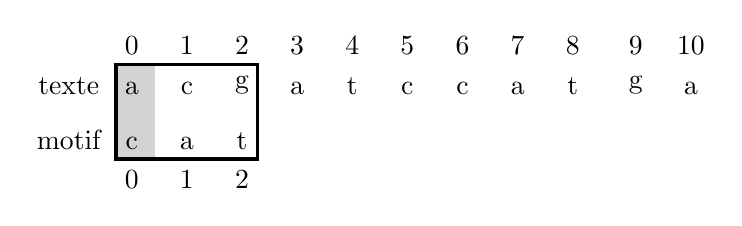
\begin{tikzpicture}
        \fill[LightGray] (1.9,0.5)--(2.4,0.5) -- (2.4,-0.7) -- (1.9,-0.7) -- cycle;
        \foreach \a/\b in {2.1/0,2.8/1,3.5/2,4.2/3,4.9/4,5.6/5,6.3/6,7/7,7.7/8,8.5/9,9.2/10}
            {\node[anchor=south] at (\a,0.5) {\b};}
        \node[anchor=south] at(1.3,0){texte};
        \foreach \a/\b in {2.1/a,2.8/c,3.5/g,4.2/a,4.9/t,5.6/c,6.3/c,7/a,7.7/t,8.5/g,9.2/a}
            {\node[anchor=south] at (\a,0) {\b};}

        \node[anchor=south] at(1.3,-0.7){motif};
        \foreach \a/\b in {2.1/c,2.8/a,3.5/t}
            {\node[anchor=south] at (\a,-0.7) {\b};}
        \foreach \a/\b in {2.1/0,2.8/1,3.5/2}
            {\node[anchor=south] at (\a,-1.2) {\b};}
        \draw[very thick] (1.9,0.5)--(3.7,0.5) -- (3.7,-0.7) -- (1.9,-0.7) -- cycle;
    \end{tikzpicture}
\end{center}

\end{frame}
\begin{frame}
    \frametitle{}

    \begin{center}
        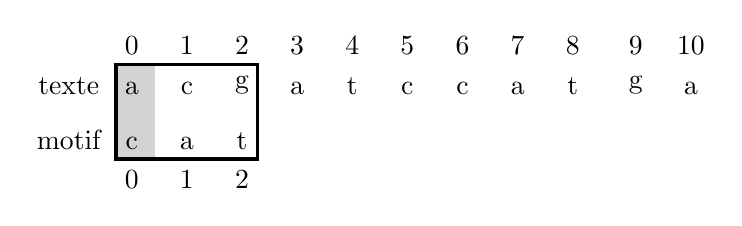
\begin{tikzpicture}
            \fill[LightGray] (1.9,0.5)--(2.4,0.5) -- (2.4,-0.7) -- (1.9,-0.7) -- cycle;
            \foreach \a/\b in {2.1/0,2.8/1,3.5/2,4.2/3,4.9/4,5.6/5,6.3/6,7/7,7.7/8,8.5/9,9.2/10}
                {\node[anchor=south] at (\a,0.5) {\b};}
            \node[anchor=south] at(1.3,0){texte};
            \foreach \a/\b in {2.1/a,2.8/c,3.5/g,4.2/a,4.9/t,5.6/c,6.3/c,7/a,7.7/t,8.5/g,9.2/a}
                {\node[anchor=south] at (\a,0) {\b};}
    
            \node[anchor=south] at(1.3,-0.7){motif};
            \foreach \a/\b in {2.1/c,2.8/a,3.5/t}
                {\node[anchor=south] at (\a,-0.7) {\b};}
            \foreach \a/\b in {2.1/0,2.8/1,3.5/2}
                {\node[anchor=south] at (\a,-1.2) {\b};}
            \draw[very thick] (1.9,0.5)--(3.7,0.5) -- (3.7,-0.7) -- (1.9,-0.7) -- cycle;
        \end{tikzpicture}
        \captionof{figure}{Première comparaison: pas de correspondance}
    \end{center}
\begin{center}
    \framebox{Décalage de la fenêtre}
\end{center}
\end{frame}
\begin{frame}
    \frametitle{}

    \begin{center}
        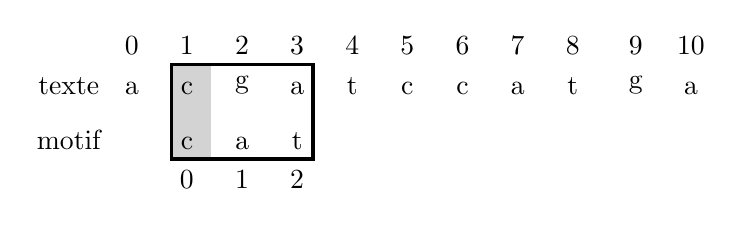
\begin{tikzpicture}
            \fill[LightGray] (2.6,0.5)--(3.1,0.5) -- (3.1,-0.7) -- (2.6,-0.7) -- cycle;
            \foreach \a/\b in {2.1/0,2.8/1,3.5/2,4.2/3,4.9/4,5.6/5,6.3/6,7/7,7.7/8,8.5/9,9.2/10}
                {\node[anchor=south] at (\a,0.5) {\b};}
            \node[anchor=south] at(1.3,0){texte};
            \foreach \a/\b in {2.1/a,2.8/c,3.5/g,4.2/a,4.9/t,5.6/c,6.3/c,7/a,7.7/t,8.5/g,9.2/a}
                {\node[anchor=south] at (\a,0) {\b};}
    
            \node[anchor=south] at(1.3,-0.7){motif};
            \foreach \a/\b in {2.8/c,3.5/a,4.2/t}
                {\node[anchor=south] at (\a,-0.7) {\b};}
            \foreach \a/\b in {2.8/0,3.5/1,4.2/2}
                {\node[anchor=south] at (\a,-1.2) {\b};}
            \draw[very thick] (2.6,0.5)--(4.4,0.5) -- (4.4,-0.7) -- (2.6,-0.7) -- cycle;
        \end{tikzpicture}
        \captionof{figure}{Première comparaison: correspondance}
    \end{center}

\end{frame}
\begin{frame}
    \frametitle{}

    \begin{center}
        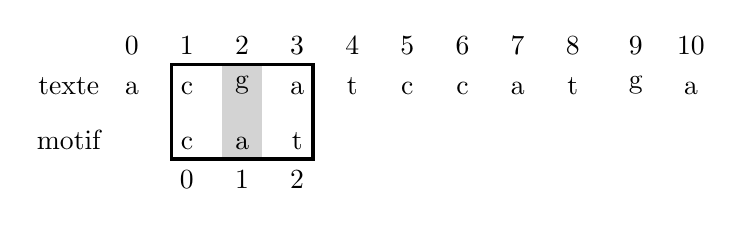
\begin{tikzpicture}
            \fill[LightGray] (3.25,0.5)--(3.75,0.5) -- (3.75,-0.7) -- (3.25,-0.7) -- cycle;
            \foreach \a/\b in {2.1/0,2.8/1,3.5/2,4.2/3,4.9/4,5.6/5,6.3/6,7/7,7.7/8,8.5/9,9.2/10}
                {\node[anchor=south] at (\a,0.5) {\b};}
            \node[anchor=south] at(1.3,0){texte};
            \foreach \a/\b in {2.1/a,2.8/c,3.5/g,4.2/a,4.9/t,5.6/c,6.3/c,7/a,7.7/t,8.5/g,9.2/a}
                {\node[anchor=south] at (\a,0) {\b};}
    
            \node[anchor=south] at(1.3,-0.7){motif};
            \foreach \a/\b in {2.8/c,3.5/a,4.2/t}
                {\node[anchor=south] at (\a,-0.7) {\b};}
            \foreach \a/\b in {2.8/0,3.5/1,4.2/2}
                {\node[anchor=south] at (\a,-1.2) {\b};}
            \draw[very thick] (2.6,0.5)--(4.4,0.5) -- (4.4,-0.7) -- (2.6,-0.7) -- cycle;
        \end{tikzpicture}
        \captionof{figure}{Deuxième comparaison: pas de correspondance}
    \end{center}
    \begin{center}
        \framebox{Décalage de la fenêtre}
    \end{center}
\end{frame}

\subsection{Implémentation}
\begin{frame}
    \frametitle{Implémentation}

    \begin{activite}
        \begin{enumerate}
            \item Écrire la fonction \textbf{\texttt{recherche\_naive(texte: str, motif: str) $\rightarrow$ int}} qui renvoie la position du \emph{motif} dans le \emph{texte} ou -1 s'il n'est pas présent.
            \item Estimer la complexité temporelle de cet algorithme dans le pire des cas: le motif n'est pas présent dans le texte.
        \end{enumerate}
    \end{activite}

\end{frame}
\begin{frame}[fragile]
    \frametitle{Correction}
\begin{center}
\begin{lstlisting}[language=Python , basicstyle=\ttfamily\small, xleftmargin=0.2em, xrightmargin=0em]
def recherche_naive(texte: str, motif: str) -> int:
    """
    renvoie la position du motif dans le texte
    -1 s'il n'est pas présent
    """
    # dernière position = taille(texte) - taille(motif)
    for i in range(len(texte)-len(motif)+1):
        j = 0
        while j < len(motif) and 
                motif[j] == texte[i+j]:
            j += 1
        # correspondance sur toute la fenêtre
        if j == len(motif): 
            return i
    return -1
\end{lstlisting}
\end{center}

\end{frame}

\begin{frame}
    \frametitle{Correction}
Imaginons le cas: 
    \begin{center}
        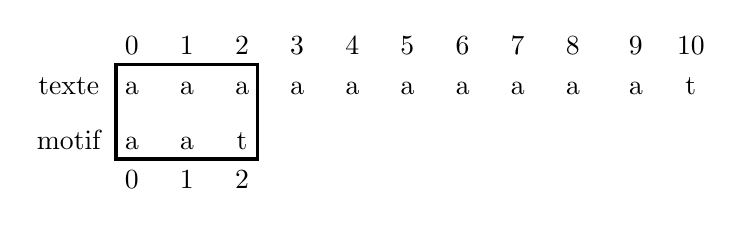
\begin{tikzpicture}
            \foreach \a/\b in {2.1/0,2.8/1,3.5/2,4.2/3,4.9/4,5.6/5,6.3/6,7/7,7.7/8,8.5/9,9.2/10}
                {\node[anchor=south] at (\a,0.5) {\b};}
            \node[anchor=south] at(1.3,0){texte};
            \foreach \a/\b in {2.1/a,2.8/a,3.5/a,4.2/a,4.9/a,5.6/a,6.3/a,7/a,7.7/a,8.5/a,9.2/t}
                {\node[anchor=south] at (\a,0) {\b};}
    
            \node[anchor=south] at(1.3,-0.7){motif};
            \foreach \a/\b in {2.1/a,2.8/a,3.5/t}
                {\node[anchor=south] at (\a,-0.7) {\b};}
            \foreach \a/\b in {2.1/0,2.8/1,3.5/2}
                {\node[anchor=south] at (\a,-1.2) {\b};}
            \draw[very thick] (1.9,0.5)--(3.7,0.5) -- (3.7,-0.7) -- (1.9,-0.7) -- cycle;
        \end{tikzpicture}
    \end{center}
\begin{itemize}
    \item On vérifie toute la fenêtre à chaque fois.
    \item À chaque \textbf{non correspondance} la fenêtre avance de 1. 
    \item La complexité dépend de la taille du texte et de celle du motif.
\end{itemize}
\note{$O(P.S)$}
\end{frame}
\section{Approche plus efficace: Boyer-Moore}
\begin{frame}
    \frametitle{Boyer-Moore}

    \begin{itemize}
        \item<1-> 1970: algorithme de Knuth-Morris-Pratt. $O(T+M)$
        \item <2-> 1977: algorithme de Boyer-Moore.
        \begin{itemize}
            \item meilleur des cas: $O(T/M)$
            \item pire des cas: $O(T+M)$
        \end{itemize} 
        \item <3-> 1980: Horspool propose une version simplifiée de l'algorithme de Boyer-Moore. $O(T)$
    \end{itemize}
\note[item]{évoquera la complexité de Boyer-Moore en fin de cours}
\note[item]{version Horspool est simplifiée mais pas forcément aussi efficace que BM}
\end{frame}
\subsection{Recherche à l'envers}
\begin{frame}
    \frametitle{Recherche à l'envers}

    La première idée de cet algorithme est de commencer la recherche \textbf{en partant de la fin du motif}.
% on parcourt toujours la chaîne de gauche à droite
\begin{center}
    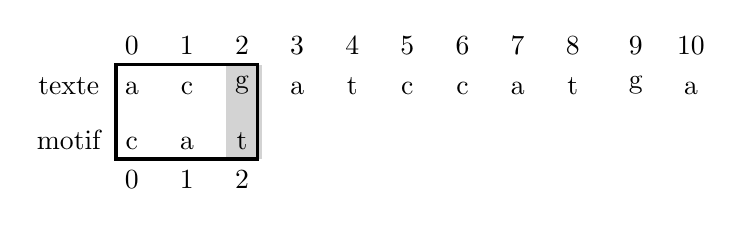
\begin{tikzpicture}
        \fill[LightGray] (3.3,0.5)--(3.75,0.5) -- (3.75,-0.7) -- (3.3,-0.7) -- cycle;
        \foreach \a/\b in {2.1/0,2.8/1,3.5/2,4.2/3,4.9/4,5.6/5,6.3/6,7/7,7.7/8,8.5/9,9.2/10}
            {\node[anchor=south] at (\a,0.5) {\b};}
        \node[anchor=south] at(1.3,0){texte};
        \foreach \a/\b in {2.1/a,2.8/c,3.5/g,4.2/a,4.9/t,5.6/c,6.3/c,7/a,7.7/t,8.5/g,9.2/a}
            {\node[anchor=south] at (\a,0) {\b};}

        \node[anchor=south] at(1.3,-0.7){motif};
        \foreach \a/\b in {2.1/c,2.8/a,3.5/t}
            {\node[anchor=south] at (\a,-0.7) {\b};}
        \foreach \a/\b in {2.1/0,2.8/1,3.5/2}
            {\node[anchor=south] at (\a,-1.2) {\b};}
        \draw[very thick] (1.9,0.5)--(3.7,0.5) -- (3.7,-0.7) -- (1.9,-0.7) -- cycle;
    \end{tikzpicture}
    \captionof{figure}{Première comparaison: pas de correspondance}
    \label{depart}
\end{center}

\end{frame}
\begin{frame}
    \frametitle{}

    \begin{aretenir}[Remarque]
        Pour l'instant cette approche ne semble par apporter d'amélioration par rapport à l'algorithme précédent.
    \end{aretenir}

\end{frame}

\subsection{Décalages par sauts}
\begin{frame}
    \frametitle{Décalage par sauts}

    Le motif ne contient pas la lettre \textbf{g} (la dernière lettre de la fenêtre).

    \begin{center}
        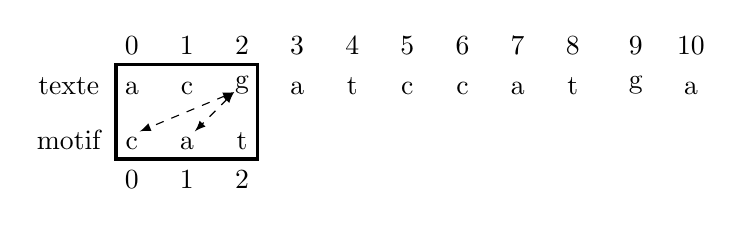
\begin{tikzpicture}
            
            \foreach \a/\b in {2.1/0,2.8/1,3.5/2,4.2/3,4.9/4,5.6/5,6.3/6,7/7,7.7/8,8.5/9,9.2/10}
                {\node[anchor=south] at (\a,0.5) {\b};}
            \node[anchor=south] at(1.3,0){texte};
            \foreach \a/\b in {2.1/a,2.8/c,3.5/g,4.2/a,4.9/t,5.6/c,6.3/c,7/a,7.7/t,8.5/g,9.2/a}
                {\node[anchor=south] at (\a,0) {\b};}
    
            \node[anchor=south] at(1.3,-0.7){motif};
            \foreach \a/\b in {2.1/c,2.8/a,3.5/t}
                {\node[anchor=south] at (\a,-0.7) {\b};}
            \foreach \a/\b in {2.1/0,2.8/1,3.5/2}
                {\node[anchor=south] at (\a,-1.2) {\b};}
            \draw[very thick] (1.9,0.5)--(3.7,0.5) -- (3.7,-0.7) -- (1.9,-0.7) -- cycle;
            \draw[<->,>=latex,dashed] (3.4,0.15) -- (2.9,-0.35);
            \draw[<->,>=latex,dashed] (3.4,0.15) -- (2.2,-0.35);
        \end{tikzpicture}
        \captionof{figure}{Comparaisons inutiles}
        \label{depart1}
    \end{center}

\end{frame}
\begin{frame}
    \frametitle{}

    \begin{center}
        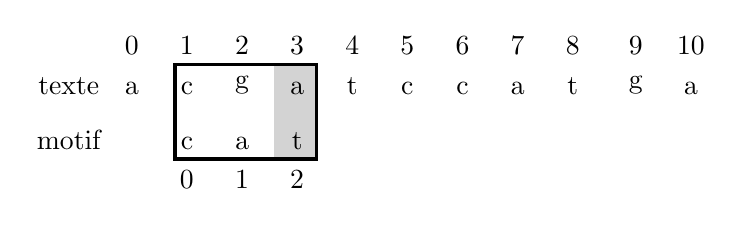
\begin{tikzpicture}
            \fill[LightGray] (3.9,0.5)--(4.45,0.5) -- (4.45,-0.7) -- (3.9,-0.7) -- cycle;
            \foreach \a/\b in {2.1/0,2.8/1,3.5/2,4.2/3,4.9/4,5.6/5,6.3/6,7/7,7.7/8,8.5/9,9.2/10}
                {\node[anchor=south] at (\a,0.5) {\b};}
            \node[anchor=south] at(1.3,0){texte};
            \foreach \a/\b in {2.1/a,2.8/c,3.5/g,4.2/a,4.9/t,5.6/c,6.3/c,7/a,7.7/t,8.5/g,9.2/a}
                {\node[anchor=south] at (\a,0) {\b};}
    
            \node[anchor=south] at(1.3,-0.7){motif};
            \foreach \a/\b in {2.8/c,3.5/a,4.2/t}
                {\node[anchor=south] at (\a,-0.7) {\b};}
            \foreach \a/\b in {2.8/0,3.5/1,4.2/2}
                {\node[anchor=south] at (\a,-1.2) {\b};}
            \draw[very thick] (2.65,0.5)--(4.45,0.5) -- (4.45,-0.7) -- (2.65,-0.7) -- cycle;
        \end{tikzpicture}
        \captionof{figure}{Comparaison inutile}
        \label{inutile1}
    \end{center}

\end{frame}
\begin{frame}
    \frametitle{}

    \begin{center}
        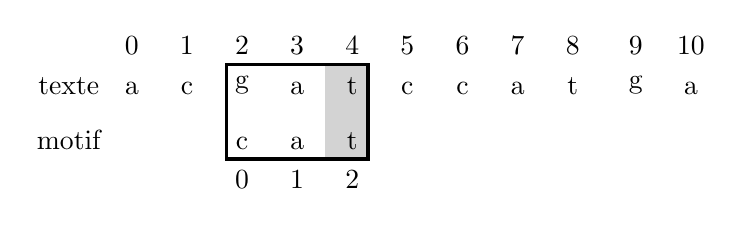
\begin{tikzpicture}
            \fill[LightGray] (4.55,0.5)--(5.1,0.5) -- (5.1,-0.7) -- (4.55,-0.7) -- cycle;
            \foreach \a/\b in {2.1/0,2.8/1,3.5/2,4.2/3,4.9/4,5.6/5,6.3/6,7/7,7.7/8,8.5/9,9.2/10}
                {\node[anchor=south] at (\a,0.5) {\b};}
            \node[anchor=south] at(1.3,0){texte};
            \foreach \a/\b in {2.1/a,2.8/c,3.5/g,4.2/a,4.9/t,5.6/c,6.3/c,7/a,7.7/t,8.5/g,9.2/a}
                {\node[anchor=south] at (\a,0) {\b};}
    
            \node[anchor=south] at(1.3,-0.7){motif};
            \foreach \a/\b in {3.5/c,4.2/a,4.9/t}
                {\node[anchor=south] at (\a,-0.7) {\b};}
            \foreach \a/\b in {3.5/0,4.2/1,4.9/2}
                {\node[anchor=south] at (\a,-1.2) {\b};}
            \draw[very thick] (3.3,0.5)--(5.1,0.5) -- (5.1,-0.7) -- (3.3,-0.7) -- cycle;
        \end{tikzpicture}
        \captionof{figure}{Comparaison inutile}
        \label{inutile2}
    \end{center}

\end{frame}
\begin{frame}
    \frametitle{}

    On peut donc directement décaler le motif à l'indice 3 du texte.
\begin{center}
    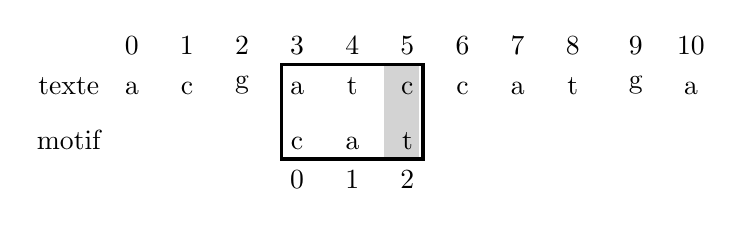
\begin{tikzpicture}
        \fill[LightGray] (5.3,0.5)--(5.75,0.5) -- (5.75,-0.7) -- (5.3,-0.7) -- cycle;
        \foreach \a/\b in {2.1/0,2.8/1,3.5/2,4.2/3,4.9/4,5.6/5,6.3/6,7/7,7.7/8,8.5/9,9.2/10}
            {\node[anchor=south] at (\a,0.5) {\b};}
        \node[anchor=south] at(1.3,0){texte};
        \foreach \a/\b in {2.1/a,2.8/c,3.5/g,4.2/a,4.9/t,5.6/c,6.3/c,7/a,7.7/t,8.5/g,9.2/a}
            {\node[anchor=south] at (\a,0) {\b};}

        \node[anchor=south] at(1.3,-0.7){motif};
        \foreach \a/\b in {4.2/c,4.9/a,5.6/t}
            {\node[anchor=south] at (\a,-0.7) {\b};}
        \foreach \a/\b in {4.2/0,4.9/1,5.6/2}
            {\node[anchor=south] at (\a,-1.2) {\b};}
        \draw[very thick] (4,0.5)--(5.8,0.5) -- (5.8,-0.7) -- (4,-0.7) -- cycle;
    \end{tikzpicture}
    \captionof{figure}{Décalage par saut}
    \label{saut0}
\end{center}

\end{frame}
\begin{frame}
    \frametitle{}

    On n'observe pas de correspondance par contre la lettre \textbf{c} existe dans le motif. On va donc le décaler pour les faire coïncider.

    \begin{center}
        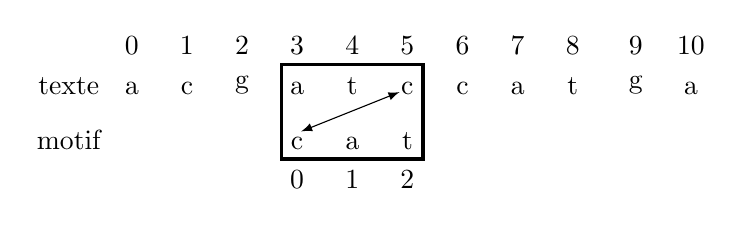
\begin{tikzpicture}
            \foreach \a/\b in {2.1/0,2.8/1,3.5/2,4.2/3,4.9/4,5.6/5,6.3/6,7/7,7.7/8,8.5/9,9.2/10}
                {\node[anchor=south] at (\a,0.5) {\b};}
            \node[anchor=south] at(1.3,0){texte};
            \foreach \a/\b in {2.1/a,2.8/c,3.5/g,4.2/a,4.9/t,5.6/c,6.3/c,7/a,7.7/t,8.5/g,9.2/a}
                {\node[anchor=south] at (\a,0) {\b};}
    
            \node[anchor=south] at(1.3,-0.7){motif};
            \foreach \a/\b in {4.2/c,4.9/a,5.6/t}
                {\node[anchor=south] at (\a,-0.7) {\b};}
            \foreach \a/\b in {4.2/0,4.9/1,5.6/2}
                {\node[anchor=south] at (\a,-1.2) {\b};}
            \draw[very thick] (4,0.5)--(5.8,0.5) -- (5.8,-0.7) -- (4,-0.7) -- cycle;
            \draw[<->,>=latex] (5.5,0.15) -- (4.25,-0.35);
        \end{tikzpicture}
        \captionof{figure}{Nouvelle situation}
        \label{saut1}
    \end{center}
\end{frame}
\begin{frame}
    \frametitle{}

    \begin{center}
        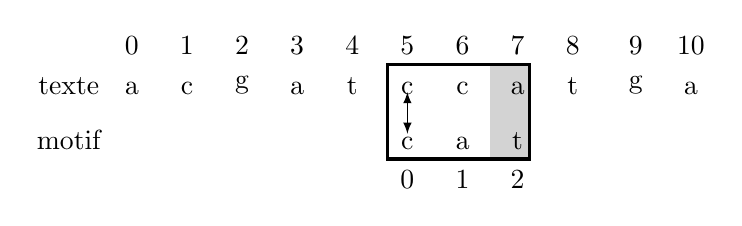
\begin{tikzpicture}
            \fill[LightGray] (6.65,0.5)--(7.15,0.5) -- (7.15,-0.7) -- (6.65,-0.7) -- cycle;
            \foreach \a/\b in {2.1/0,2.8/1,3.5/2,4.2/3,4.9/4,5.6/5,6.3/6,7/7,7.7/8,8.5/9,9.2/10}
                {\node[anchor=south] at (\a,0.5) {\b};}
            \node[anchor=south] at(1.3,0){texte};
            \foreach \a/\b in {2.1/a,2.8/c,3.5/g,4.2/a,4.9/t,5.6/c,6.3/c,7/a,7.7/t,8.5/g,9.2/a}
                {\node[anchor=south] at (\a,0) {\b};}
    
            \node[anchor=south] at(1.3,-0.7){motif};
            \foreach \a/\b in {5.6/c,6.3/a,7/t}
                {\node[anchor=south] at (\a,-0.7) {\b};}
            \foreach \a/\b in {5.6/0,6.3/1,7/2}
                {\node[anchor=south] at (\a,-1.2) {\b};}
            \draw[very thick] (5.35,0.5)--(7.15,0.5) -- (7.15,-0.7) -- (5.35,-0.7) -- cycle;
            \draw[<->,>=latex] (5.6,-0.38)--(5.6,0.15);
        \end{tikzpicture}
        \captionof{figure}{Décalage par saut}
        \label{saut2}
    \end{center}

\end{frame}
\begin{frame}
    \frametitle{}

    \begin{aretenir}[]
        On décale la position de recherche dans le texte en fonction de la dernière lettre de la fenêtre.
    \end{aretenir}
\note[item]{et de sa présence éventuelle dans le motif}
\note[item]{il existe variante \emph{bad char}: on décale en fonction du caractère qui ne correspond pas}
\end{frame}

\subsection{Prétraitement du motif}
\begin{frame}
    \frametitle{Prétraitement du motif}

    \begin{aretenir}[]
        Pour pouvoir décaler par saut, il faut connaître la dernière position de chaque lettre dans le motif. Le prétraitement consiste à calculer le décalage à appliquer pour amener chaque caractère du motif à la place du dernier caractère.
    \end{aretenir}
    \begin{center}
        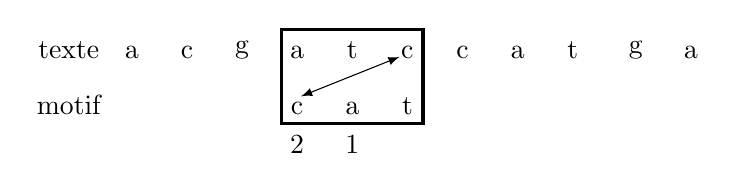
\begin{tikzpicture}
            \node[anchor=south] at(1.3,0){texte};
            \foreach \a/\b in {2.1/a,2.8/c,3.5/g,4.2/a,4.9/t,5.6/c,6.3/c,7/a,7.7/t,8.5/g,9.2/a}
                {\node[anchor=south] at (\a,0) {\b};}
    
            \node[anchor=south] at(1.3,-0.7){motif};
            \foreach \a/\b in {4.2/c,4.9/a,5.6/t}
                {\node[anchor=south] at (\a,-0.7) {\b};}
            \foreach \a/\b in {4.2/2,4.9/1}
                {\node[anchor=south] at (\a,-1.2) {\b};}
            \draw[very thick] (4,0.5)--(5.8,0.5) -- (5.8,-0.7) -- (4,-0.7) -- cycle;
            \draw[<->,>=latex] (5.5,0.15) -- (4.25,-0.35);
        \end{tikzpicture}
        \captionof{figure}{Calculs des décalages}

    \end{center}
\end{frame}
\begin{frame}
    \frametitle{}

    \begin{aretenir}[Remarque]
        On ne regarde pas la dernière position de la clé (la lettre \emph{t} ici). Sinon la distance associée serait nulle et on resterait sur place après l’avoir lue dans le texte.
        
    \end{aretenir}
    \begin{center}
        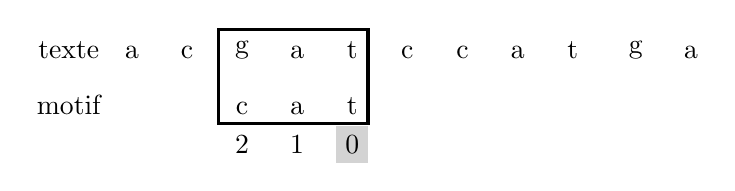
\begin{tikzpicture}
            \node[anchor=south] at(1.3,0){texte};
            \foreach \a/\b in {2.1/a,2.8/c,3.5/g,4.2/a,4.9/t,5.6/c,6.3/c,7/a,7.7/t,8.5/g,9.2/a}
                {\node[anchor=south] at (\a,0) {\b};}
    
            \node[anchor=south] at(1.3,-0.7){motif};
            \foreach \a/\b in {3.5/c,4.2/a,4.9/t}
                {\node[anchor=south] at (\a,-0.7) {\b};}
            \foreach \a/\b in {3.5/2,4.2/1}
                {\node[anchor=south] at (\a,-1.2) {\b};}
            \draw[very thick] (3.2,0.5)--(5.1,0.5) -- (5.1,-0.7) -- (3.2,-0.7) -- cycle;
            \node[anchor=south,fill=LightGray] at(4.9,-1.2){0};
        \end{tikzpicture}
        \captionof{figure}{Sauf la dernière lettre}

    \end{center}
\note{attention t pourrait être présent ailleurs dans motif $\rightarrow$ on prend en compte alors}
\end{frame}
\begin{frame}
\begin{aretenir}[]
Dans le cas de la répétition d'un caractère, on garde la distance la plus courte.
\end{aretenir}
    \begin{center}
        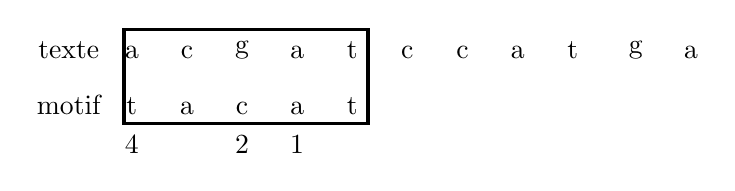
\begin{tikzpicture}
            \node[anchor=south] at(1.3,0){texte};
            \foreach \a/\b in {2.1/a,2.8/c,3.5/g,4.2/a,4.9/t,5.6/c,6.3/c,7/a,7.7/t,8.5/g,9.2/a}
                {\node[anchor=south] at (\a,0) {\b};}
    
            \node[anchor=south] at(1.3,-0.7){motif};
            \foreach \a/\b in {2.1/t,2.8/a,3.5/c,4.2/a,4.9/t}
                {\node[anchor=south] at (\a,-0.7) {\b};}
            \foreach \a/\b in {2.1/4,2.8/ ,3.5/2,4.2/1}
                {\node[anchor=south] at (\a,-1.2) {\b};}
            \draw[very thick] (2,0.5)--(5.1,0.5) -- (5.1,-0.7) -- (2,-0.7) -- cycle;
            
        \end{tikzpicture}
        \captionof{figure}{Répétition dans le motif}

    \end{center}
\note{on fait coïncider le premier \emph{t} du motif avec la dernière lettre de la fenêtre}
\end{frame}
\begin{frame}
    \frametitle{}

    \begin{activite}
        Écrire la fonction \textbf{\texttt{pretraitement\_decalages(motif: str) $\rightarrow$ dict}} qui associe chaque lettre du motif (sauf la dernière) à son décalage.
    \end{activite}

\end{frame}
\begin{frame}[fragile]
    \frametitle{Correction}

\begin{center}
\begin{lstlisting}[language=Python , basicstyle=\ttfamily\small, xleftmargin=0.2em, xrightmargin=0em]
def pretraitement_decalages(motif: str) -> dict:
    """
    renvoie le dictionnaire des décalages à appliquer
    pour chaque lettre du motif (sauf dernière)
    """
    decalages = dict()
    # on s'arrête à l'avant dernière lettre du motif
    for i in range(len(motif)-1):
        # la distance est mise à jour en cas de répétition
        decalages[motif[i]] = len(motif)-1-i
    return decalages
\end{lstlisting}
\end{center}

\end{frame}
\subsection{Algorithme de Boyer-Moore (simplifié - version Horspool)}
\begin{frame}[fragile]
    \frametitle{Algorithme de Boyer-Moore}


    L'algorithme de Boyer-Moore s'écrit alors:
\begin{center}
\begin{lstlisting}[language=Bash, basicstyle=\small\ttfamily, xleftmargin=2em, xrightmargin=2em]
Créer le tableau des décalages
Tant qu'on n'est pas à la fin du texte
    Comparer le motif à la position du texte
    Si le motif est présent
        Renvoyer la position
    Sinon
        Décaler la fenêtre
Renvoyer -1 si le motif n'est pas présent
\end{lstlisting}
\captionof{code}{Algorithme de Boyer-Moore (version Horspool)}
\label{algo}
\end{center}
\note{Horspool: en 1980, version simplifiée de Boyer-Moore; il existe plusieurs versions.}
\end{frame}

\begin{frame}
    \frametitle{}

    \begin{activite}
        \begin{enumerate}
            \item Écrire la fonction \textbf{\texttt{compare(texte: str, position: int, motif: str) $\rightarrow$ bool}} qui renvoie \texttt{\textbf{True}} si le motif est présent à la position \textbf{\texttt{i}} du texte.
            \item Écrire la fonction \textbf{\texttt{decalage\_fenetre(decalages: dict, taille: int, lettre: str) $\rightarrow$ int}} qui renvoie le décalage à appliquer pour faire coïncider le motif à la dernière \emph{lettre} de la fenêtre. Si la lettre n'est pas présente, la \texttt{\textbf{taille}} du motif est renvoyée.
            \item Écrire alors la fonction \textbf{\texttt{boyer\_moore(texte: str, motif: str) $\rightarrow$ int}} qui renvoie la position du motif dans le texte et -1 sinon.
        \end{enumerate}
    \end{activite}

\end{frame}
\begin{frame}[fragile]
    \frametitle{Correction}

\begin{center}
\begin{lstlisting}[language=Python , basicstyle=\ttfamily\small, xleftmargin=0.2em, xrightmargin=0em]
def compare(texte: str, position: int, motif: str) -> bool:
    # position de la dernière lettre de la fenêtre
    en_cours = position+len(motif)-1
    # parcours de la fenêtre à l'envers
    for i in range(len(motif)-1, -1, -1):
        if not(texte[en_cours] == motif[i]):
            return False
        else:
            en_cours -= 1
    return True
\end{lstlisting}
\end{center}

\end{frame}
\begin{frame}[fragile]
\begin{center}
\begin{lstlisting}[language=Python , basicstyle=\ttfamily\small, xleftmargin=0.2em, xrightmargin=0em]
def decalage_fenetre(decalages: dict, taille: int, lettre: str) -> int:
    for cle, val in decalages.items():
        if cle == lettre:
            return val
    # si la lettre n'est pas dans le dico (= le motif)
    return taille
\end{lstlisting}
\end{center}

\end{frame}
\begin{frame}[fragile]

\begin{center}
\begin{lstlisting}[language=Python , basicstyle=\ttfamily\small, xleftmargin=0.2em, xrightmargin=0em]
def decalage_fenetre2(decalages: dict, taille: int, lettre: str) -> int:
    # la méthode get renvoie une valeur par défaut si elle ne trouve pas la clé
    return decalages.get(lettre, taille)
\end{lstlisting}
\begin{lstlisting}[language=Python , basicstyle=\ttfamily\small, xleftmargin=0.2em, xrightmargin=0em]
def decalage_fenetre3(decalages: dict, taille: int, lettre: str) -> int:
    try:
        res = decalages[lettre]
    except KeyError:
        res = taille
    return res
\end{lstlisting}
\captionof{code}{Variantes}
\label{CODE}
\end{center}

\end{frame}
\begin{frame}[fragile]
\begin{center}
\begin{lstlisting}[language=Python , basicstyle=\ttfamily\small, xleftmargin=0.2em, xrightmargin=0em]
def boyer_moore(texte: str, motif: str) -> int:
    decalages = pretraitement_decalages(motif)
    i = 0
    while i <= len(texte)-len(motif):
        # si on trouve le motif
        if compare(texte, i, motif):
            return i
        else:
            # sinon on décale (en fonction de la dernière lettre de la fenêtre)
            decale = decalage_fenetre(
                            decalages, 
                            len(motif), 
                            texte[i+len(motif)-1]
                            )
            i += decale
    # si on sort de la boucle, on n'a rien trouvé
    return -1
\end{lstlisting}
\end{center}

\end{frame}
% d'autres versions (bad char, good suffix)
\subsection{Complexité}
\begin{frame}
    \frametitle{Complexité}

    Intuitivement l'algorithme semble plus rapide que la version naïve car il ne teste pas toutes les lettres du texte.
\begin{center}
    \begin{tabular}{*{15}{c}}
        a&a&a&a&b&a&a&a&a&b&a&a&a&a&b\\
        c&c&c&c&c&&&&&&&&&&\\
    \end{tabular}
    \captionof{figure}{Un cas représentatif}
\end{center}

\end{frame}
\begin{frame}
    \frametitle{}

    \begin{center}
        \begin{tabular}{*{15}{c}}
            a&a&a&a&b&a&a&a&a&b&a&a&a&a&b\\
            &c&c&c&c&c&&&&&&&&&\\
        \end{tabular}
    \end{center}
    \begin{center}
        \begin{tabular}{*{15}{c}}
            a&a&a&a&b&a&a&a&a&b&a&a&a&a&b\\
            &&c&c&c&c&c&&&&&&&&\\
        \end{tabular}
        \captionof{figure}{Algorithme naïf}
    \end{center}
\begin{aretenir}[Observation]
L'algorithme naïf effectue 10 décalages.
\end{aretenir}
\end{frame}
\begin{frame}
    \frametitle{}

    \begin{center}
        \begin{tabular}{*{15}{c}}
            a&a&a&a&b&a&a&a&a&b&a&a&a&a&b\\
            &&&&&c&c&c&c&c&&&&&\\
        \end{tabular}
    \end{center}
    \begin{center}
        \begin{tabular}{*{15}{c}}
            a&a&a&a&b&a&a&a&a&b&a&a&a&a&b\\
            &&&&&&&&&&c&c&c&c&c\\
        \end{tabular}
        \captionof{figure}{Algorithme de Boyer-Moore}
    \end{center}
    \begin{aretenir}[Observation]
        L'algorithme de Boyer-Moore-Horspool effectue 3 décalages.
        \end{aretenir}
\end{frame}
\begin{frame}
    \frametitle{}

    \begin{aretenir}[Remarques]
        \begin{itemize}
            \item Dans le meilleur des cas, la complexité temporelle de l'algorithme est $O(T/M)$ où T est la taille du texte et M celle du motif.
            \item Plus le motif est long plus l'algorithme est rapide.
            \item Le prétraitement a un coût (temporel et spatial) mais qui est grandement compensé.
        \end{itemize}
        \end{aretenir}
\note[item]{complexité sous-linéaire!}
\note[item]{Naïf $O(T.M)$}
\note[item]{Complexité moyenne: $O(3.M)$ démontrée par Richard Cole en 1991.}
\note[item]{coût spatial si alphabet grand.}

\end{frame}
\begin{frame}
    \frametitle{Cas critique}

    \begin{center}
        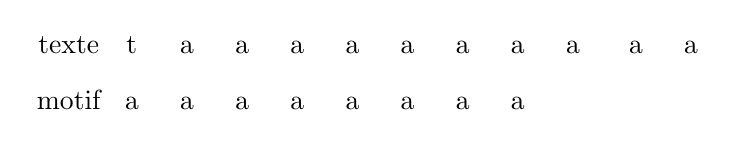
\begin{tikzpicture}
            \node[anchor=south] at(1.3,0){texte};
            \foreach \a/\b in {2.1/t,2.8/a,3.5/a,4.2/a,4.9/a,5.6/a,6.3/a,7/a,7.7/a,8.5/a,9.2/a}
                {\node[anchor=south] at (\a,0) {\b};}
    
            \node[anchor=south] at(1.3,-0.7){motif};
            \foreach \a/\b in {2.1/a,2.8/a,3.5/a,4.2/a,4.9/a,5.6/a,6.3/a,7/a}
                {\node[anchor=south] at (\a,-0.7) {\b};}
            
        \end{tikzpicture}
    \end{center}
    \vspace*{3em}
    \begin{center}
        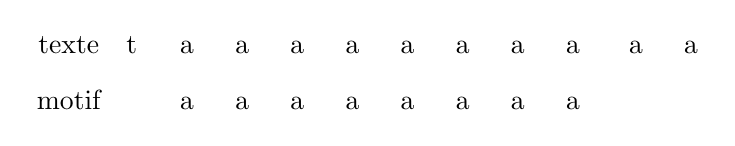
\begin{tikzpicture}
            \node[anchor=south] at(1.3,0){texte};
            \foreach \a/\b in {2.1/t,2.8/a,3.5/a,4.2/a,4.9/a,5.6/a,6.3/a,7/a,7.7/a,8.5/a,9.2/a}
                {\node[anchor=south] at (\a,0) {\b};}
    
            \node[anchor=south] at(1.3,-0.7){motif};
            \foreach \a/\b in {2.8/a,3.5/a,4.2/a,4.9/a,5.6/a,6.3/a,7/a,7.7/a}
                {\node[anchor=south] at (\a,-0.7) {\b};}
            
        \end{tikzpicture}
        \captionof{figure}{Cas critique}

    \end{center}
\note{.}
\end{frame}
\begin{frame}
    \frametitle{}

    \begin{aretenir}[Remarque]
        En plus d'un traitement du mauvais caractère, la version complète de l'algorithme de Boyer-Moore recherche des bons suffixes dans le motif.
    \end{aretenir}

\end{frame}
\end{document}